\documentclass[a4paper,12pt]{article}

\usepackage{multirow}
\usepackage[left=1cm,right=1cm,
top=2cm,bottom=2cm,bindingoffset=0cm]{geometry}
\usepackage[utf8]{inputenc}
\usepackage[russian]{babel}
\usepackage[T2A]{fontenc}
\usepackage{amsfonts,longtable, amssymb, amsmath}
\usepackage{graphicx}
\usepackage{wrapfig}
\usepackage{hyperref}
%\urlstyle{same}
\usepackage{pdfpages}
%\usepackage{pscyr}
\usepackage[normalem]{ulem}  % для зачекивания текста
\usepackage{ulem}
\graphicspath{{pictures/}}
\DeclareGraphicsExtensions{.pdf,.png,.jpg, .svg}
\usepackage{pgfplots}
\pgfplotsset{compat=1.12}
\usepackage{fancyhdr}
\pagestyle{fancy}
\fancyhead{}
\fancyhead[LO]{} 
\fancyhead[CO]{}
\fancyhead[RO]{}

\usepackage{graphicx,url}

\usepackage[russian]{babel}   
%\usepackage[latin1]{inputenc}  
\usepackage[utf8]{inputenc}  
\usepackage{verbatim}

\begin{document}

\section*{Ответы, день 1}

\begin{enumerate}
     	\item Ниже приведены эскизы графиков заданных функций.
     	\begin{figure}[h!]
     		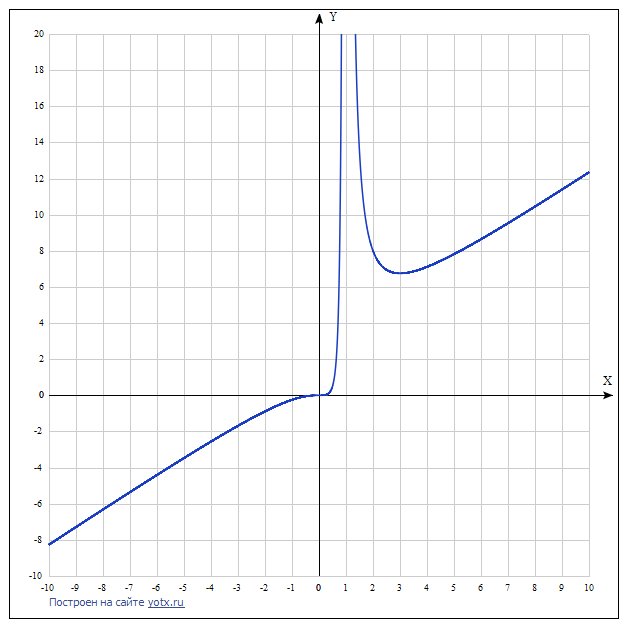
\includegraphics[scale=0.35]{1(1).png}
     		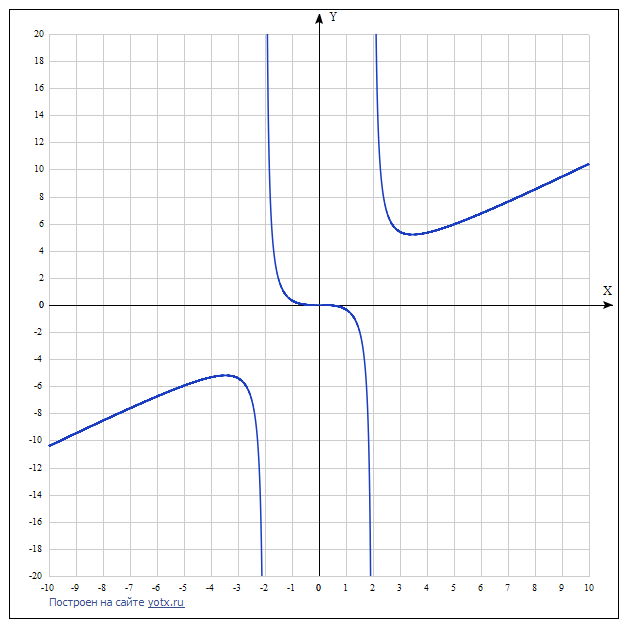
\includegraphics[scale=0.35
     		]{1(2).png}
     		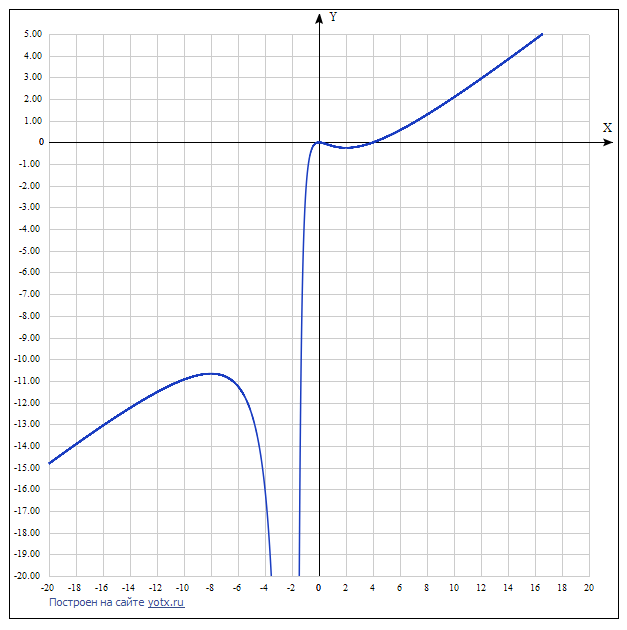
\includegraphics[scale=0.35]{1(3).png}
     		\caption{Эскизы графиков к задаче №1 (от пункта 1 к пункту 3 слева направо)}
		\end{figure}
     	
     	\item Аналогично предыдущей задаче:
     	\begin{figure}[h!]
     		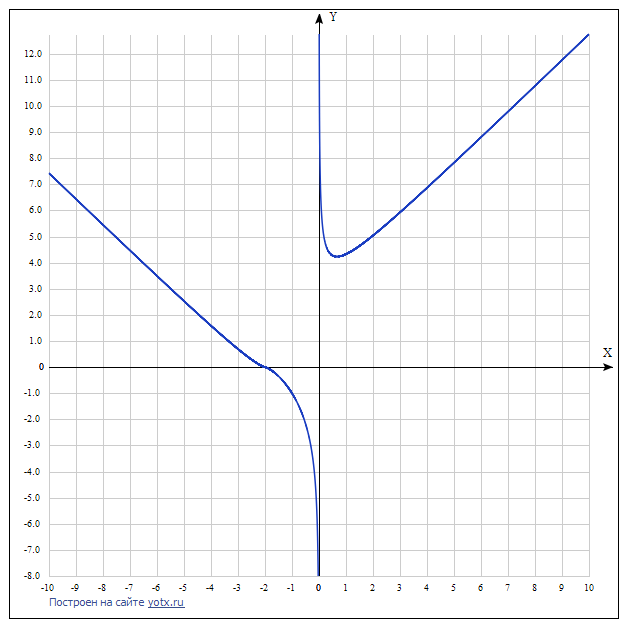
\includegraphics[scale=0.35]{2(1).png}
     		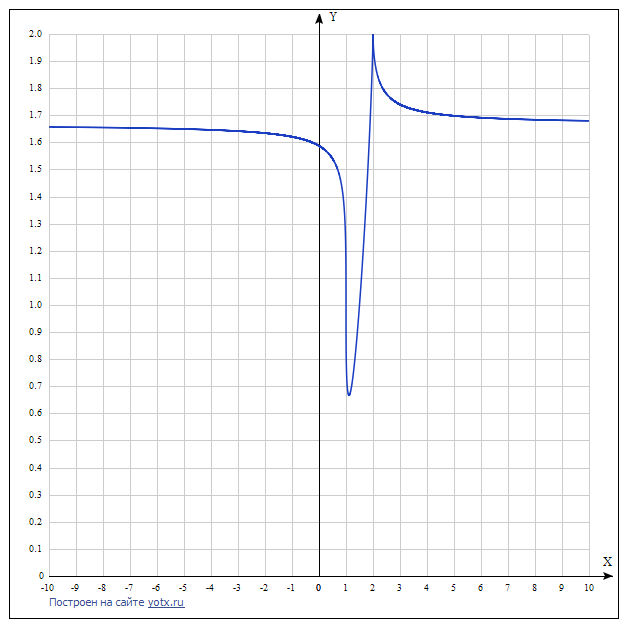
\includegraphics[scale=0.35]{2(2).png}
     		\caption{Эскизы графиков к задаче №2 (от пункта 1 к пункту 2 слева направо)}
		\end{figure}
     	
     	\item $k_{min} = \dfrac{1}{9 \sqrt{2}}$.
     	
     	\item $k = \dfrac{1}{\sqrt{5}}$. \\
     	\textit{Примечание.} Не нужно находить общую формулу для кривизны! Достаточно вычислить все необходимые производные в заданной точке, и только затем применить формулу.
     	 
     	\item $k = \dfrac{7}{\sqrt{2}}$, $R = \dfrac{\sqrt{2}}{7}$.
\end{enumerate}

\end{document}